\documentclass[a4paper,11.5pt]{article}
\usepackage[latin1]{inputenc}
\usepackage[T1]{fontenc}
\usepackage[english]{babel}
\usepackage{graphicx}
\usepackage{amsmath}
\usepackage{amsfonts}
\usepackage{multirow}
\usepackage{booktabs}
\usepackage{bbold}
\usepackage{mathtools}
\usepackage{mathrsfs}
\usepackage{enumitem}
\usepackage{array}
\usepackage{float}

\setlength{\parindent}{0pt}
\DeclarePairedDelimiter{\floor}{\lfloor}{\rfloor}
\DeclarePairedDelimiter{\ceil}{\lceil}{\rceil}

\newcommand{\vt}{\boldsymbol}

\title{Digital Communications - HW4}
\author{Jacopo Pegoraro, Edoardo Vanin}
\date{04/06/2018}

\begin{document}

\maketitle

We want to implement and evaluate the performances of two modulation schemes in the case of uncoded and coded bits. The first system we consider is a matched filter/DFE receiver with single carrier modulation. The information signal in this case is transmitted through the channel and equalized at the receiver by canceling the ISI due to the postcursors of the total impulse response with feedback, while the ISI due to the precursors is reduced by the feedforward filter $c$. In the case of OFDM instead we use a multi-carrier approach and we carry out the equalization by using the \emph{cyclic prefix} method. 

\section*{System setup}

The setup of the system is carried out differently for the uncoded and coded cases. The starting point is a sequence of bits $b_l$ on sampling time $T_{bit}$, produced by a PN sequence with parameter $r=20$ and length $L=2^r-1$ repeated once.

\subsection*{Uncoded}

In the uncoded case the sequence $b_l$ directly mapped into a sequence of QPSK symbols $a_k$ at sampling time $T_a=2T_{bit}$ through a bitmap function that uses Gray coding. At the receiver the detected sequence will pass through an inverse bitmap before the computation of the probability of bit error $P_{bit}$.

\subsection*{Coded}

In the coded case the sequence is first coded using an irregular LDPC code with rate $1/2$ and a codelength of $N = 64800$. This operation produces a sequence of bits $c_m$ with double the length of $b_l$ and sampling time $T_{cod}$. To improve the performances by reducing the effect of burst errors, $c_m$ is passed to an interleaver $43 \times 41$ in which we write the input bits by row and read them by column to perform a scramble.

At this point the resulting bit sequence $c_p'$ at $T_a = 2T_{cod}$ is transmitted using the single carrier and OFDM schemes. At the receiver, once the detection has taken place, the reverse operations are carrier out to derive the detected bit sequence $\hat{b}_l$ and compute $P_{bit}$. In particular a LDPC decoder and a deinterleaver $41\times 43$ are used. It is important to remark hat in the coded case the LDPC algorithm works with \emph{soft information}, so we pass to it not the detected bits, but the log-likelihood ratios $l_m$ for which we give proper expression later.

Where $y_k$ is the dectected symbol in case of DFE equalization and the DFT of the recivers it in case of OFDM. The $\sigma_w$ is the noise variance per component.

\section*{Single Carrier with DFE}

The system takes a sequence of input symbols $a_k$ at sampling time $T_a=2T_{cod}$ and applies an upsampling of factor 4, obtaining $a_k'$ at $T_a/4$. This new sequence is then filtered by $q_c$ as described by the following difference equation:
\begin{equation}\label{eq:q_c}
s_c(nT_a/4) = 0.67 s_c((n-1)T_a/4) + 0.7424 a_{n-5}
\end{equation}
After the filtering white noise is added. From the following relations we can derive $\sigma_w^2$, the variance of the complex valued Gaussian noise:
\begin{equation}
\Gamma = \frac{M_{s_c}}{N_0\frac{1}{T_a}} = \frac{\sigma_a^2 E_{q_c}}{\sigma_w^2} \longrightarrow \sigma_w^2 = \frac{\sigma_a^2 E_{q_c}}{\Gamma} = 2\sigma_I^2
\end{equation}
where $\sigma_I^2$ is the variance per component. In addition we can also compute the PSD as $N_0=\sigma_w^2 T_c=\sigma_w^2/4$, because the sampling time $T_c$ at which we add the noise is $T_a/4$.
In figure \ref{fig:qc} we plot the impulse response and the frequency response of the filter $q_c$.

\begin{figure}[H]
	\begin{center}   
		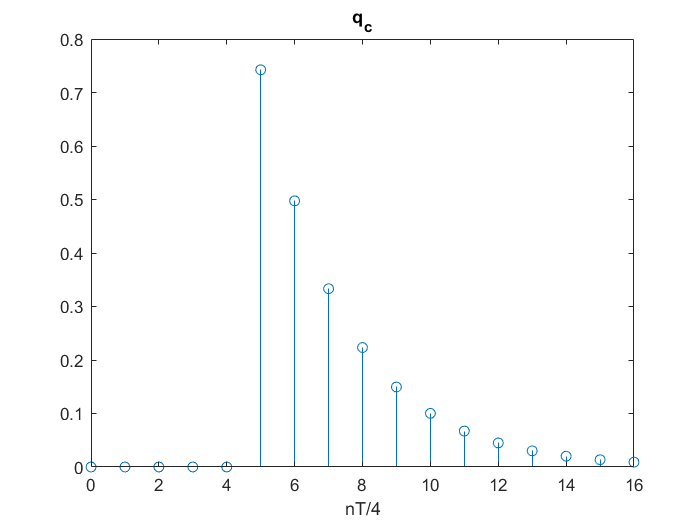
\includegraphics[width=10cm]{figs/q_c.png}  
		\caption{Impulse response of the filter $q_c$ at $T_c$.}
		\label{fig:qc}
	\end{center}
\end{figure} 

At the receiver we have a matched filter $g_{M}$, obtained from $q_c$ as $g_M=q_c^*(t_0-t)$. For simplicity in the last formula we have denoted the filters as is they were defined on continuous time while in the actual simulation they are at $T_a/4$. 

The output of the matched filter is then sampled at $T_a$ starting from an initial offset called \emph{timing phase} $t_0$. In our case the choice of $t_0$ is made easy by the presence of the matched filter, as we can just choose the value $\bar{t}_0$, multiple of $T_a/4$, that is the index of the peak of the correlation between $q_c$ and $g_M$, then $t_0$ will be equal to $\bar{t}_0 T_a/4$. Following this reasoning we chose $\bar{t}_0=16$ (17 with Matlab indexing), equal also to the index of the last sample of $g_M$.

We equalize with a DFE, that is made of two filters called feedforward and feedback filter denoted by $c$ and $b$. The feedforward filter has the role of equalizing only the precursors of the overall impulse response, while the ISI due to postcursors will be canceled by filter $b$ positioned on a feedback loop between the output of the threshold detector and its input. 


The computation of the optimal filters $c$ and $b$ is carried out using the Wiener filter approach. The relation between the input random process and the output is:
\begin{equation}
\begin{split}
y_k &= x_{FF,k} + x_{FB,k} \\
&= \sum_{i=0}^{M_1-1}c_ix_{k-i} + \sum_{j=1}^{M_2}b_ja_{k-D-j}
\end{split} 
\end{equation}
where $M_1$ is the order of the feedforward filter, $M_2$ is the order of the feedback filter and $a_{k-D}$ are the already detected past symbols fed back through $b$. Defining postcursors and precursors as in point A, we have that we can apply the Wiener-Hopf equations on the process:
\begin{equation} \label{eq:yk}
y_k = \sum_{i=0}^{M_1-1}c_i \left(x_{k-i}-\sum_{j=1}^{M_2}h_{j+D-i}a_{k-j-D} \right)
\end{equation}

The result can be easily computed as $c_{opt} = \vt{R}^{-1}\vt{p}$ once we find the autocorrelation matrix $\vt{R}$ and the correlation vector $\vt{p}$, expressed as \cite{nevio<3}:

\begin{equation} \label{eq:wienerR}
\mathbf{[R]}_{p,q} = \sigma_a^2 \left( \sum_{j=-N_1}^{N_2}h_jh^*_{j-(p-q)}-\sum_{j=1}^{M_2}h_{j+D-q}h^*_{j+d-p} \right) + r_{\tilde{w}}(p-q)
\end{equation}
\begin{equation} \label{eq:wienerp}
\mathbf{[p]}_p = \sigma_a^2 h^*_{D-p} \quad\quad\quad\quad\quad\quad p = 0,1,\dots,M_1-1
\end{equation}

where for a QPSK scheme $\sigma_a^2=2$ because it is the sum of two orthogonal components each with power $1$. The values of $r_{\tilde{w}}$ are the result of the autocorrelation of the noise after being filtered by $g_M$, so being the noise white we have $r_{\tilde{w}}(n)=N_0r_{g_M}(nT)$. At this point we can define the overall impulse response up to the threshold detector $\psi = h*c_{opt}$ and derive the optimal coefficients for filter $b$ as $b_i=-\psi_{i+D}$ for $i=1,\dots,M_2$.

The value of the cost function $J_{min}$ obtained using these the optimal filters is :
\begin{equation} \label{eq:jmin}
J_{min} = \sigma^2_a \left( 1-\sum_{l=0}^{M_1-1} c_{opt,l}h_{D-l}\right)
\end{equation}

Again the parameters to choose are the order of filter $c$, $M_1$, and the delay introduced $D$. This is because the order of $b$ can be chosen in such a way that all the postcursors are canceled by the feedback: $M_2=N_2+M_1-D-1$, and also the expression of the autocorrelation matrix significantly simplifies. The choice is carried out by selecting the values that minimize the functional $J_{min}$, as homework 3 being $M_1=5$ and $D=4$, and consequently $M_2=4$ because $N_2=4$. Before the decision point we scale down the output of the equalizer $y_k$ by the amplitude of the peak of the overall impulse response $\psi_D$, obtaining $\bar{y}_k = a_k + \frac{v_k}{|\psi_D|}$ that is coherent with the input modulation symbols.

The following table summarizes the chosen parameters for the single carrier system:

\begin{table}[htbp]
	\begin{center}
		\begin{tabular}{cccccc}
			\toprule
			$N_1$ & $N_2$ & $M_1$ & $M_2$ & $D$ & $\bar{t}_0$ \\
			\midrule
			 4  &  4  & 5 & 4  & 4 & 16 \\
			\bottomrule
		\end{tabular}
	\end{center}
	\label{tab:sumup}
	\caption{Choices for the various parameters for the DFE with respect to the number of precursors and postcursors of $h$, $N_1$ and $N_2$.}
\end{table} 

For the simulation with coding we first P/S convert the log-likelihood ratios as:

\begin{equation}
l'_{2k} =- \frac{2 \Re\{y_k\}}{\sigma_{I}^2} \quad \quad
l'_{2k+1}= - \frac{2 \Im\{y_k\}}{\sigma_{I}^2}
\end{equation}

where we have the noise variance per component $\sigma_I^2=\frac{\sigma_{w_c}^2}{2}$ where  $\sigma_{w_c}^2 = \frac{J_{min}-\sigma_a^2 |1-\psi_D|^2}{|\psi_D|^2}$ is the noise variance after the feedforward equalizer filter $c$, scaled by the amplitude of the peak of the overall impulse response $\psi_D$ . The resulting series of values is deinterleaved (see the first section for details on how the interleaver is built) and passed to the LDPC decoder that works with \emph{soft information}.

\section*{OFDM with cyclic prefix}

The system considered in this case is represented in figure \ref{fig:ofdm_schema}:
 
\begin{figure}[H]
	\begin{center}   
		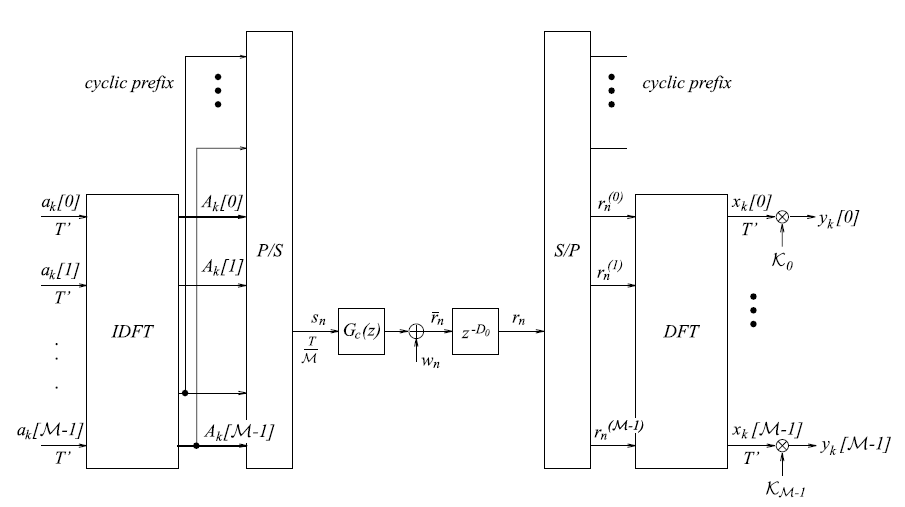
\includegraphics[width=\textwidth]{figs/OFDM_schema.png} 
		\caption{Block diagram of the OFDM system with the cyclic prefix method.}
		\label{fig:ofdm_schema}
	\end{center}
\end{figure}

The input sequence of symbols $a_k$ is arranged in a matrix with $\mathcal{M}=512$ rows and on these blocks of length $\mathcal{M}$ we compute the IDFT to obtain the sequence $A_k[i]$ for $i=0,\dots , \mathcal{M}-1$. At this point we used the cyclic prefix method to perform equalization: a prefix of length $N_{px}$ taken from the end of the block obtained from IDFT is repeated on top of the same block. In this way, choosing $N_{px}\geq N_c-1$ (where $N_c$ is the length of the channel impulse response) the data of the next block will be separated from the present one by $N_c-1$ or more samples, that is enough to fill the channel and not have any ICI between consecutive blocks. In our specific case $N_c=19$ (see the overall impulse response $h$ in figure \ref{fig:h}) so we can take $N_{px}=18$.
This addition cause a reduction in the rate of the transmission that depends on how long is $N_{px}$. Indeed the time at which the block of input data is accepted is $T_{block} = T_{OFMD} \cdot (\mathcal{M} + N_{px}) = T_a \cdot \frac{\mathcal{M} + N_{px}}{\mathcal{M}}$. In the following description, we assume $T_{OFDM} = 1$ to simplify the interpretation of the plots.
 At the receiver the additional $A_k[i]$ with $i=\mathcal{M}-1-N_{px},\dots ,\mathcal{M}-1$ can be just discarded. The DFT is computed to retrieve the original symbols and each subchannel is rescaled by a factor $\mathcal{K}_i = \frac{1}{\mathcal{H}_i}$ where $\mathcal{H}_i$ for $i=0, \dots, \mathcal{M}-1$ is the DFT  computed on $\mathcal{M}$ points of the impulse response $h$ (see figure \ref{fig:H}).

\subsection*{OFDM channel}

The channel, represented as a single block in figure \ref{fig:ofdm_schema} contains all blocks depicted in figure \ref{fig:ofdm_channel_schema}

\begin{figure}[H]
	\begin{center}   
		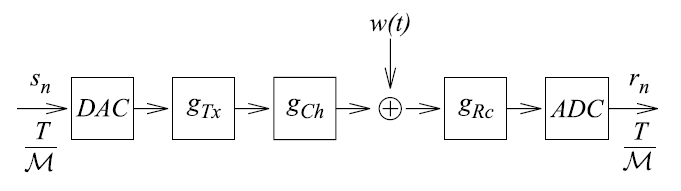
\includegraphics[width=10cm]{figs/OFDM_channel_schema.png} 
		\caption{Channel + transmitter and receiver filters in OFDM.}
		\label{fig:ofdm_channel_schema}
	\end{center}
\end{figure}

where in our case $g_{tx}$ and $g_{Rc}$ are taken both as square root raised cosine filters, and the channel impulse response is the $q_c$ used also for the single carrier channel: 
\begin{equation}\label{eq:q_c}
s_c(nT_{OFDM}/4) = 0.67 s_c((n-1)T_{OFDM}/4) + 0.7424 a_{n-5}
\end{equation}
The system takes a sequence of input symbols $s_k$ at sampling time $T_{OFDM}=T_{block}/(M + N_{px})$ and applies an upsampling of factor 4, obtaining $a_k'$ at $T_c = T_{OFDM}/4$. This new sequence is then filtered by $g_{\sqrt{rcos}}$ where the impulse response is described by the following equation sampled at time $T_c=T_{OFDM}/4$ and truncated where the amplitude of the taps was lower than $10^{-2} \cdot \max\{g_{\sqrt{rcos}}\}$. 
.
\begin{equation}\label{eq:g_rcos}
g_{\sqrt{rcos}}(n) = \frac{\sin\left[\pi\left(1 - \rho\right)\frac{n}{T_c}\right] + 4\rho\frac{n}{T_c}\cos\left[\pi\left(1 - \rho\right)\frac{n}{T_c}\right]}{\pi\left[1-\left(4\rho\frac{n}{T_c}\right)^2\right]\frac{n}{T_c}}
\end{equation}
The result can be seen in figure \ref{fig:gimp_rcos}:


\begin{figure}[H]
	\begin{center}   
		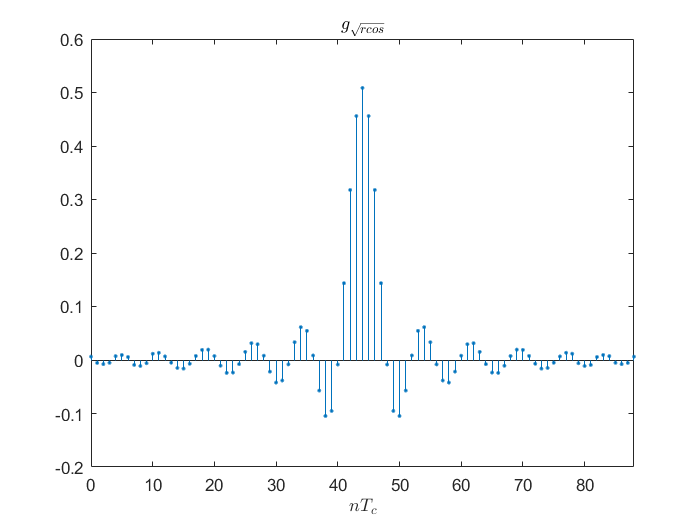
\includegraphics[width=10cm]{figs/gimp_rcos.png} 
		\caption{Impulse response of the square root raised cosine filter $g_{\sqrt{rcos}}$.}
		\label{fig:gimp_rcos}
	\end{center}
\end{figure}

And the following picture represents the frequency response $|\mathcal{G}_{\sqrt{rcos}}|$:

\begin{figure}[H]
	\begin{center}   
		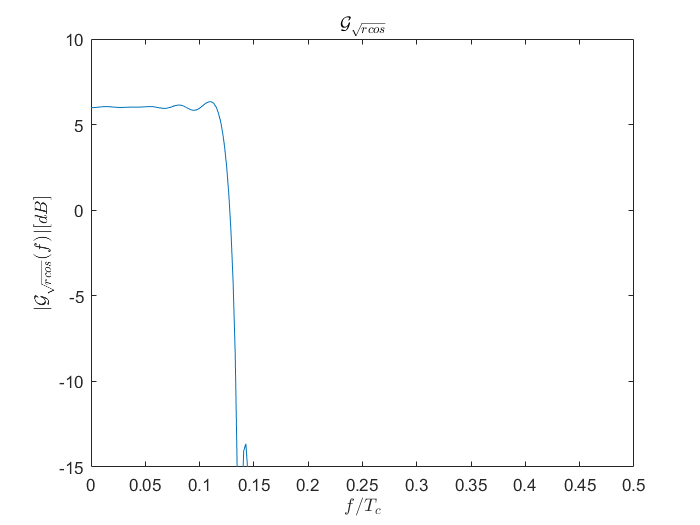
\includegraphics[width=10cm]{figs/G_rcos.png} 
		\caption{Frequency response of the square root raised cosine filter.}
		\label{fig:Grcos}
	\end{center}
\end{figure}

After the convolution with the transmit filter, we send the data through the channel with the impulse response given by (\ref{eq:q_c}) and white noise is added. From the following relations we can derive $\sigma_w^2$, the variance of the complex valued Gaussian noise:
\begin{equation}
\Gamma = \frac{M_{s_c}}{N_0\frac{1}{T_OFDM}} = \frac{\sigma_s^2 E_{g_{\sqrt{rcos}} * q_c}}{\sigma_w^2} \longrightarrow \sigma_w^2 = \frac{\sigma_a^2 E_{g_{\sqrt{rcos}} *q_c}}{\mathcal{M}\Gamma} = 2\sigma_I^2
\end{equation}

where we used the relation $\sigma_s^2 = \frac{\sigma_a^2}{\mathcal{M}}$ \cite{nevio<3}.

At the receiver we have another $g_{\sqrt{rcos}}$ with the impulse response given by (\ref{eq:g_rcos}).
The output of the matched filter is then sampled at $T_{OFDM}$ starting from an initial offset called \emph{timing phase} $t_0$. We can just choose the value $\bar{t}_0$, multiple of $T_c=T_{OFDM}/4$ and we have chosen $\bar{t}_0=42$ (43 with Matlab indexing) because it corresponds to the peak of the overall impulse response $q_R$ at $T_c$ as we can see from the following figure:

\begin{figure}[H]
	\begin{center}   
		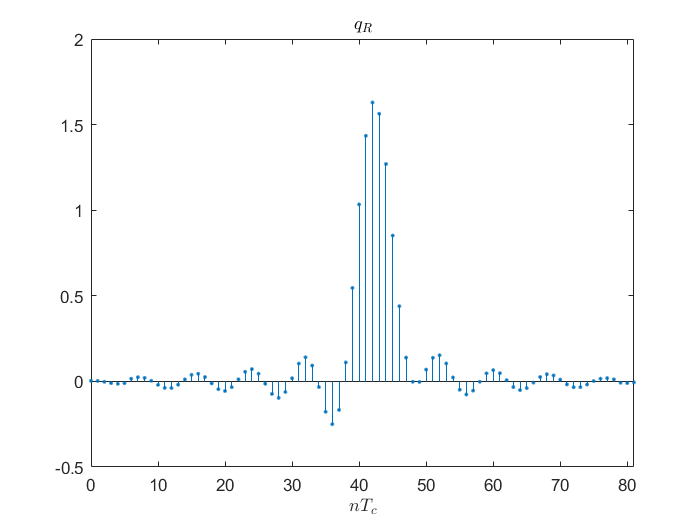
\includegraphics[width=\textwidth]{figs/q_R.png} 
		\caption{Total impulse response of the channel and receiver/transmit filters.}
		\label{fig:q_R}
	\end{center}
\end{figure}

The total impulse response obtained by convolving the three filters is depicted in figure \ref{fig:q_R} at sampling time $T_c$, and the corresponding frequency response can be seen in figure \ref{fig:Qmag_R}.

\begin{figure}[H]
	\begin{center}   
		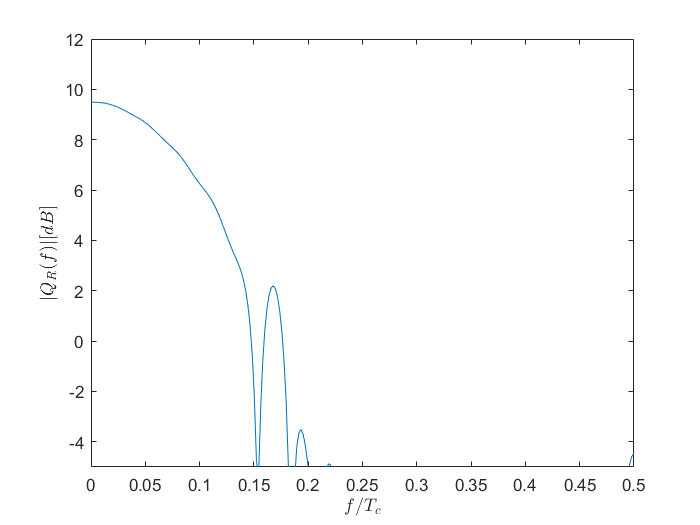
\includegraphics[width=10cm]{figs/Qmag_R.png} 
		\caption{Frequency response of the total channel and receive/transmit filters at $T_c$}
		\label{fig:Qmag_R}
	\end{center}
\end{figure}

However, if we want to derive an impulse response that relates the input of the whole transmitter+channel+receiver system, we have to work on the sampling time $T_{OFDM}$. We will call the downsampled version of $q_R$ with the appropriate timing phase $h$ (see figure \ref{fig:h}). Its DFT is instead plotted in figure \ref{fig:H}. 

\begin{figure}[H]
	\begin{center}   
		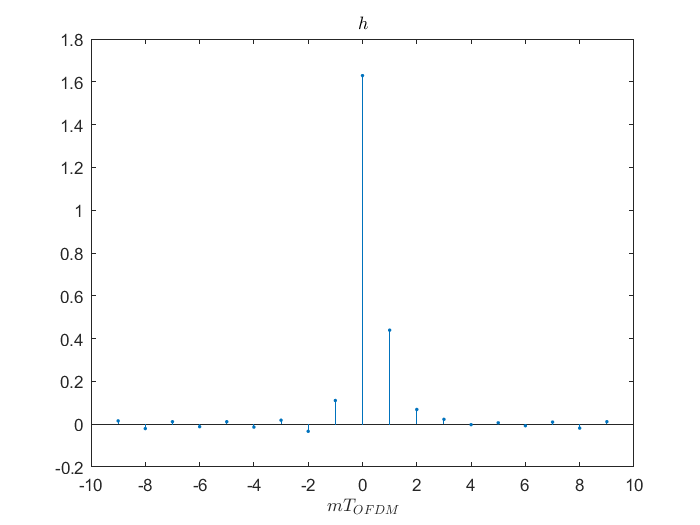
\includegraphics[width=10cm]{figs/h.png} 
		\caption{Total impulse response $h$ at $T_{OFDM}$.}
		\label{fig:h}
	\end{center}
\end{figure}



\begin{figure}[H]
	\begin{center}   
		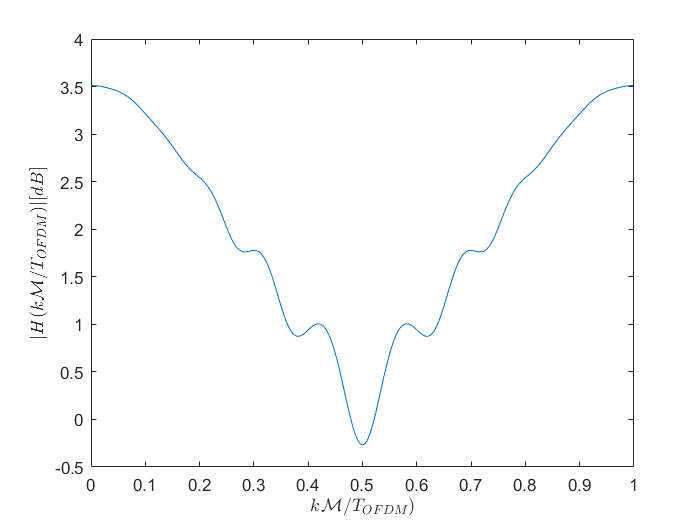
\includegraphics[width=10cm]{figs/H_mag.png} 
		\caption{Frequency response of the total system at $T_{OFDM}$.}
		\label{fig:H}
	\end{center}
\end{figure}


To improve the performance in some case it ca be useful to introduce the so called \emph{virtual carriers}, so to transmit a sequence of all zeros instead of data on subchannels with index close to $\mathcal{M}/2$. This method allows to increase the transition band of the signal $s_n$ and to simply the filters at the transmitter and receiver. However in our case the transition band of the raised cosine filters is very sharp without causing complexity problems. We tried to introduce a small number of virtual carriers $N_{vir} = 1,3,5$ but the improvement in the performances was not noticeable, at the cost of reducing the data transmitted with the same bandwidth usage. For this reason we decided to simulate the performances of our system without any virtual carrier.

The following table summarizes the parameters for the OFDM system:

\begin{table}[htbp]
	\begin{center}
		\begin{tabular}{ccc}
			\toprule
			$N_{px}$ & $N_{vir}$ &$\bar{t}_0$ \\
			\midrule
			18 & 0 & 42 \\
			\bottomrule
		\end{tabular}
	\end{center}
	\label{tab:sumup2}
	\caption{Choices for the various parameters in the OFDM system.}
\end{table} 

For the simulation with coding we first P/S convert the log-likelihood ratios for each subchannel obtained as:

\begin{equation}
l'_{2k}[i] =- \frac{2 \Re\{y_k[i]\}}{\sigma_{I,OFDM}^2} \quad \quad
l'_{2k+1}[i]= - \frac{2 \Im\{y_k[i]\}}{\sigma_{I,OFDM}^2}
\end{equation}

where we have the noise variance per component $\sigma_{I,OFDM} = \frac{\sigma_W^2}{2 \mathcal{H}_i}=\frac{\mathcal{M} \sigma_w^2}{2 \mathcal{H}_i}$, the variance of the DFT of the noise $\sigma_W^2 = \mathcal{M} \sigma_w^2$ and the output of the OFDM system for each subchannel:
\begin{equation} \label{eq:outOFDM}
 y_k[i] = a_k[i] + \frac{W_k[i]}{\mathcal{K}_i}
\end{equation}
 The resulting series of values is rearranged with the deinterleaver (see the first section for details on how the interleaver is built) and passed to the LDPC decoder that works with \emph{soft information}.

\section*{Simulation results}

The simulation has been carried out using as input a PN sequence with $r=20$ repeated, so the total length of the bit stream is $2L = 2(2^r-1) = 2097150$. In the coded case we also applied LDPC encoding and interleaving (see the first section). The obtained bits are assumed to be distributed approximately as random. Given that we have to estimate the probability for a range of values going from $10^{-1}$ to $10^{-5}$, we need to be sure that our estimate is not affected by a high variance. The estimator we chose is:
\begin{equation}
\hat{P}_{bit} = \frac{\#_{wrong}}{\#_{tx}}
\end{equation}
where $\#_{wrong}$ is the number of erroneously detected bits and $\#_{tx}$ is the total number of transmitted bits. As $\#_{tx}$ increases the estimator becomes approximately a Gaussian random variable, unbiased and with variance: $\frac{P_{bit} (1-P_{bit})}{\#_{tx}}$. This confirms that our estimate is reliable because the resulting variance will be very small, according to the empirical rule for which if we want to estimate a $P_{bit}$ of $10^{-k}$, we need to measure it transmitting around $30\cdot 10^{k}$ symbols. Indeed in our case the smallest $P_{bit}$ we need to estimate is $10^{-5}$ and so the required number of bits to have a very good estimate would be $30\cdot 10^{5}= 3000000$. We decide however to use a less stringent criterion, so to transmit at least $20\cdot 10^5$ bits, because we noticed that the resulting variance was already low enough to guarantee a good estimate and the simulation speed was greatly improved.

The results obtained for various values of the SNR are plotted in figure \ref{fig:Pbit_uncoded} for the uncoded case and \ref{fig:Pbit_coded} for the coded case.


\begin{figure}[H]
	\begin{center}   
		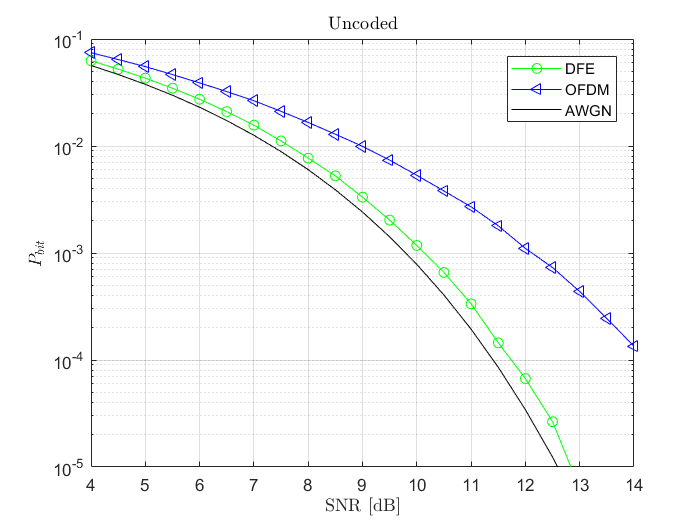
\includegraphics[width=\textwidth]{figs/Pbit_uncoded_1.png} 
		\caption{$P_{bit}$ obtained for various values of the SNR with DFE equalization and OFDM, no channel coding used.}
		\label{fig:Pbit_uncoded}
	\end{center}
\end{figure}

We can notice that in the uncoded case the performances of the DFE are better than the OFDM system. The reason for this is explained by considering equation \ref{eq:outOFDM}. If the coefficients of the channel impulse response DFT are small, we can have that the scaling done at the output of the OFDM structure enhances the noise and disturbs useful data. This problem is solved almost entirely by channel coding, because errors due to this can be corrected. Indeed in figure \ref{fig:Pbit_coded} we can see that in the coded case the situation is reversed and the OFDM performs better than the DFE.
It is also noticeable the drastic reduction of the SNR values needed to achieve the same values of the $P_{bit}$ using the LDPC. This is due to the fact that the rate is $1/2$, so the real rate of the overall system is reduced by half as we have to transmit this overhead.

\begin{figure}[H]
	\begin{center}   
		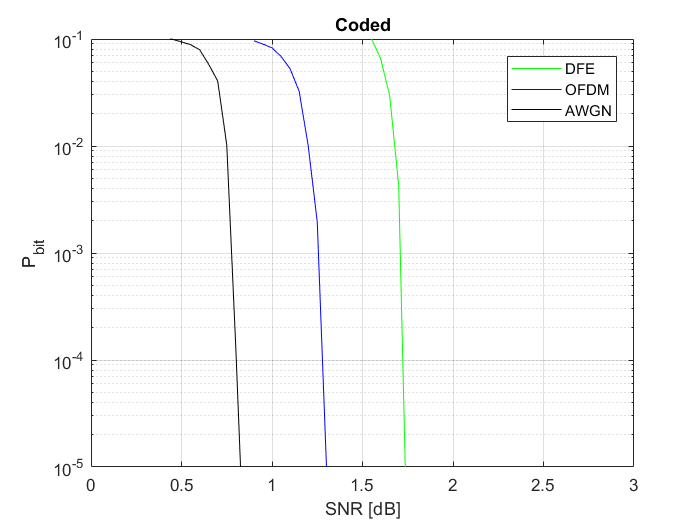
\includegraphics[width=\textwidth]{figs/Pbit_coded.png} 
		\caption{$P_{bit}$ obtained for various values of the SNR with DFE equalization and OFDM, LDPC coding has been used.}
		\label{fig:Pbit_coded}
	\end{center}
\end{figure}



 
\begin{thebibliography}{15}	
	\bibitem{nevio<3}
	Nevio Benvenuto, Giovanni Cherubini,
	\textit{Algorithms for Communication Systems and their Applications}. 
	Wiley, 2002.
\end{thebibliography}

\end{document}